\chapter{Asking a Billionaire Lawyer How to Make \$1,000,000}

This chapter follows the School of Hard Knocks interview with John Morgan as a source-conscious case study in wealth built through a professional-service business. The mathematical content is not classroom algebra on a board; it is business arithmetic: capped versus uncapped upside, risk transfer, distribution, advertising spend, legal execution, debt, and the way repeated trust becomes enterprise value. The transcript is treated as the source of claims, with curation by LazyingArt LLC through Video2Book.

\section{A Rare Route to Billionaire Status}

The opening hook is deliberately simple: we are about to meet a billionaire in Florida, and the fortune is said to have come through law. The host identifies the guest as John Morgan, attributes a net worth of about \$1.5 billion to Forbes, and frames Morgan as unusual because relatively few people become billionaires through personal injury law.

The first numerical spine of the chapter is therefore not a calculation but a set of spoken claims:

\begin{align}
N_{\mathrm{Forbes}} &\approx \$1.5\mathrm{B},\\
F_{\mathrm{annual\ fees}} &\approx \$2\mathrm{B},\\
D_{\mathrm{debt}} &= 0.
\end{align}

Here \(N_{\mathrm{Forbes}}\) denotes the host's Forbes-attributed net-worth figure, \(F_{\mathrm{annual\ fees}}\) denotes Morgan's later claim about annual fees, and \(D_{\mathrm{debt}}\) records his repeated statement that he has no debt. These quantities should be read as transcript-backed claims, not audited financial statements.

The local puzzle is now visible. A conventional law practice can become an excellent income engine, but it is usually constrained by human time, case load, and professional capacity. Morgan's first answer is that scale did not begin with a clever legal doctrine. It began with delegation, trusted partners, and sharing the profit.

\section{Scale Begins With Partners, Not Employees}

Morgan's answer to the question of how the firm grew is direct: delegate, find partners one can trust, and let them share in the business. If the firm wants great people, they must make money with the founder, not merely for the founder.

This is the first operating equation of the lecture. A founder-only practice has a bottleneck:

\begin{equation}
\mathrm{Output}_{\mathrm{solo}} \leq \mathrm{capacity}_{\mathrm{founder}}.
\end{equation}

A partnership model changes the object being built. The relevant capacity is no longer one person's working day, but the sum of reliable operators who can carry cases, make decisions, and reduce the founder's need to touch everything:

\begin{equation}
\mathrm{Output}_{\mathrm{firm}} \approx \sum_{i=1}^{n} q_i c_i,
\end{equation}

where \(c_i\) is the operating capacity of partner \(i\), and \(q_i\) is a rough trust-and-quality factor. This is not Morgan's notation; it is a compact way to express the mechanism in the interview. The point is that a law firm scales only if the people added to the system increase dependable capacity rather than merely increasing supervision cost.

\subsection{Question \& Answer}

\paragraph{Question.}
How does a law practice stop being one person's job and become a multibillion-dollar firm?

\paragraph{Answer.}
It has to cease being founder-centered. Morgan's answer is to delegate to people he trusts and share the economics with them. The key person is what he calls a ``send-delete'' person: someone who can receive a task, handle it, and let the founder delete the worry. In these notes we can treat that as a management compression function:

\begin{equation}
\mathrm{Attention\ returned} =
\mathrm{Task\ delegated}
-
\mathrm{Followup\ required}.
\end{equation}

A send-delete operator has low followup cost. That is why such people compound firm capacity.

\section{Pain, Purpose, and the First Work Ethic}

After scale, the interview moves backward into motive. Morgan says his brother Tim was paralyzed at C6--C7 when Morgan was in college, and that the way Tim was treated changed Morgan's life. He says that when he sees clients, he sees Tim, and wants to treat them the way Tim should have been treated.

This should not be flattened into a generic motivational sentence. The interview makes a sharper distinction: the business is not presented first as an abstract market opportunity, but as pain converted into a durable operating purpose. The sequence is:

\begin{enumerate}
\item A family injury creates anger at how an injured person is treated.
\item The anger becomes a reason to go to law school with a clear target.
\item The legal practice becomes a repeated promise: protect clients as Tim should have been protected.
\end{enumerate}

Morgan then connects work ethic to childhood. He says his father did not have much money, jokes that his father needed a cosigner to pay cash, and then describes paper routes and selling cards at seven years old. A paper route matters because it is daily work with no vacation. In the language of these notes, it is an early test of consistency:

\begin{equation}
\mathrm{Hustle} \sim \mathrm{daily\ obligation} + \mathrm{customer\ responsibility} + \mathrm{no\ vacation}.
\end{equation}

That equation is not meant as a law of human nature. It is a faithful reconstruction of Morgan's claim: he sees early repeated responsibility as evidence of entrepreneurial temperament.

\section{Upside, Contingency Fees, and Negotiation Silence}

The interview then pivots to law-school advice. Morgan contrasts ordinary hourly legal work with his contingency-fee model. The transcript appears to garble a few words here, but the meaning is clear: he does not want to charge by the hour because there is not enough upside for him. He gets paid if he wins.

The standard reconstruction is:

\begin{align}
R_{\mathrm{hourly}} &= r h,\\
R_{\mathrm{contingency}} &=
\begin{cases}
0, & \hbox{if the case loses},\\
\alpha S, & \hbox{if the case wins},
\end{cases}
\end{align}

where \(r\) is an hourly rate, \(h\) is billable time, \(S\) is settlement or verdict value, and \(\alpha\) is an unspecified share. The transcript does not give \(\alpha\), so we should not invent it.

The business distinction is the important part. Hourly billing gives a bounded linear model. Contingency work is riskier, but it ties revenue to outcome rather than time. Morgan's preference is not for safety; it is for upside attached to winning.

\subsection{Question \& Answer}

\paragraph{Question.}
Why reject hourly billing if hourly billing is more predictable?

\paragraph{Answer.}
Because predictability can cap the outcome. In an hourly model, the ceiling is constrained by rates, hours, staffing, and collections. In a contingency model, the firm takes downside risk in exchange for a claim on the result. Morgan's answer is not that contingency fees are always better. His narrower claim is that hourly work does not contain enough upside for the kind of firm he wanted to build.

The same section produces a negotiation rule: whoever speaks first loses. In context, this is not a mystical rule of silence. Morgan immediately translates it into listening. People who talk too much do not hear. The negotiator first sizes up the deal and the person, then acts.

A compact negotiation update rule is:

\begin{equation}
\mathrm{Offer}_{t+1}
=
f(\mathrm{information\ heard}_{t},\ \mathrm{person}_{t},\ \mathrm{deal}_{t}).
\end{equation}

If one speaks too early, the information set is smaller. Morgan's point is that listening increases the quality of the next move.

\section{Reputation, Negative Energy, and Controlled Liability}

The middle of the interview widens from deal-making to character under stress. Morgan names luck, faith, and reputation. He says successful people pat themselves on the back too much, and that one different left turn, right turn, or U-turn could have changed everything. The useful business conclusion is not fatalism; it is humility under uncertainty.

The practical rule he says he received from a mentor is: keep your word. Reputation becomes a long-horizon asset:

\begin{equation}
\mathrm{Trust}_{t+1}
=
\mathrm{Trust}_{t}
+
\mathrm{promises\ kept}_{t}
-
\mathrm{promises\ broken}_{t}.
\end{equation}

This is schematic, but it captures the interview's mechanism. Reputation is not decoration; it affects whether people keep coming back.

The conversation then introduces negative people, betrayal, and mistakes. Morgan says sometimes one must pay people to walk away, and he uses the language of cutting cancers out of the business. The phrase is harsh, but the mechanism is clear: destructive people carry an ongoing cost. Paying them to leave can be cheaper than letting them remain.

He also describes professional mistakes. When lawyers in his firm make mistakes and harm a case, he says he admits it, brings in the client, and relies on insurance and money to make the client whole.

\subsection{Question \& Answer}

\paragraph{Question.}
What happens when the firm itself causes harm?

\paragraph{Answer.}
Morgan's answer is controlled liability rather than denial. Admit the mistake, tell the client, use insurance, and take care of the client even if the client must hire a lawyer and sue the firm. In business terms, the loss is not merely legal. The larger loss would be destroying trust by hiding the mistake.

\section{The Google Law Firm and Brick-by-Brick Expansion}

After a promotional interlude from the host about proximity, mentorship, dates, pricing, and community access, the interview returns to Morgan. The next question is about competition. Morgan says competition makes people great, citing Michael Jordan as an example, and then gives the central strategic image of the lecture: he wanted to build the Google law firm.

The meaning is distribution. If Google were a law firm, Morgan says, it would be everywhere for everyone:

\begin{equation}
\mathrm{Coverage}=50\ \mathrm{states},
\qquad
\mathrm{Availability}=24/7.
\end{equation}

He adds that a person can become his client by phone in two minutes. This is a customer-access claim. It belongs in the chapter as distribution architecture, not as a legal claim about licensing or jurisdiction.

\subsection{Question \& Answer}

\paragraph{Question.}
How does a national vision avoid collapsing under its own ambition?

\paragraph{Answer.}
Morgan answers with sequence. He says he went first from Orlando to Tampa, then from Orlando to Jacksonville, then from Orlando to Naples, brick by brick. The vision is national, but the construction is local and cumulative.

\begin{figure}
\centering
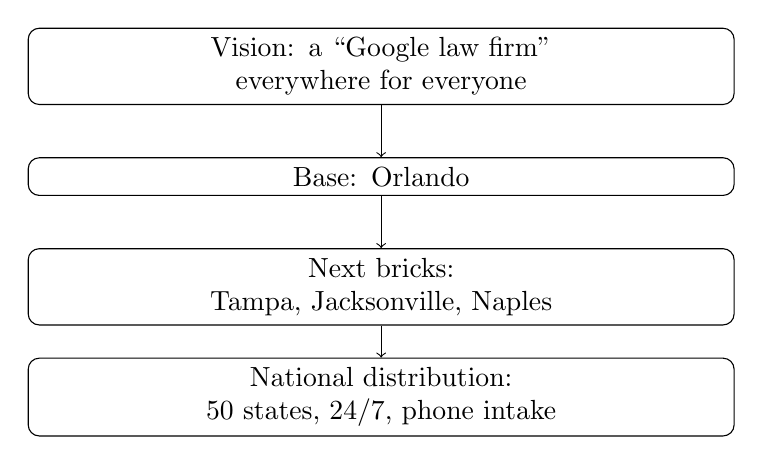
\begin{tikzpicture}[x=1cm,y=1cm]
\node[draw, text width=.72\linewidth, align=center, rounded corners] (vision) at (0,0) {Vision: a ``Google law firm''\\ everywhere for everyone};
\node[draw, text width=.72\linewidth, align=center, rounded corners] (orlando) at (0,-1.4) {Base: Orlando};
\node[draw, text width=.72\linewidth, align=center, rounded corners] (cities) at (0,-2.8) {Next bricks:\\ Tampa, Jacksonville, Naples};
\node[draw, text width=.72\linewidth, align=center, rounded corners] (national) at (0,-4.2) {National distribution:\\ 50 states, 24/7, phone intake};

\draw[->] (vision) -- (orlando);
\draw[->] (orlando) -- (cities);
\draw[->] (cities) -- (national);
\end{tikzpicture}
\caption{A transcript-grounded reconstruction of Morgan's national expansion logic: broad vision, local sequencing, then national availability.}
\end{figure}

The three little pigs metaphor appears here as a caution against weak construction. Straw and sticks do not survive a hurricane; bricks do. In these notes that means scale must be built from repeatable operating units, not one burst of attention.

\section{Marketing Catches Fish; Lawyers Cook Fish}

The strongest numerical mechanism arrives late in the interview. Morgan says he spends about \$400 million per year on advertising and that the firm did about \$5 billion in settlements and verdicts. The host observes that this is less than 10 percent. We can compute the simple ratio:

\begin{align}
A_{\mathrm{advertising}} &= \$400\mathrm{M},\\
V_{\mathrm{settlements+verdicts}} &= \$5\mathrm{B},\\
\frac{A_{\mathrm{advertising}}}{V_{\mathrm{settlements+verdicts}}}
&=
\frac{400\mathrm{M}}{5\mathrm{B}}
=
0.08
=
8\%
<
10\%.
\end{align}

This is a useful calculation, but we must be precise about what it is not. It is not a profit margin. It is not audited return on advertising. It is simply a transcript-backed comparison between stated advertising spend and stated settlements plus verdicts.

Morgan then gives the mechanism: there are two things in his business, catching fish and cooking fish. Catching fish is client acquisition: advertising, brand, and incoming demand. Cooking fish is legal execution: the lawyers who can actually get verdicts. The insurance industry, he says, knows who wins, and he names software called Colossus as part of how insurers evaluate firms and cases. The claim should be preserved as a transcript-backed institutional detail.

\begin{figure}
\centering
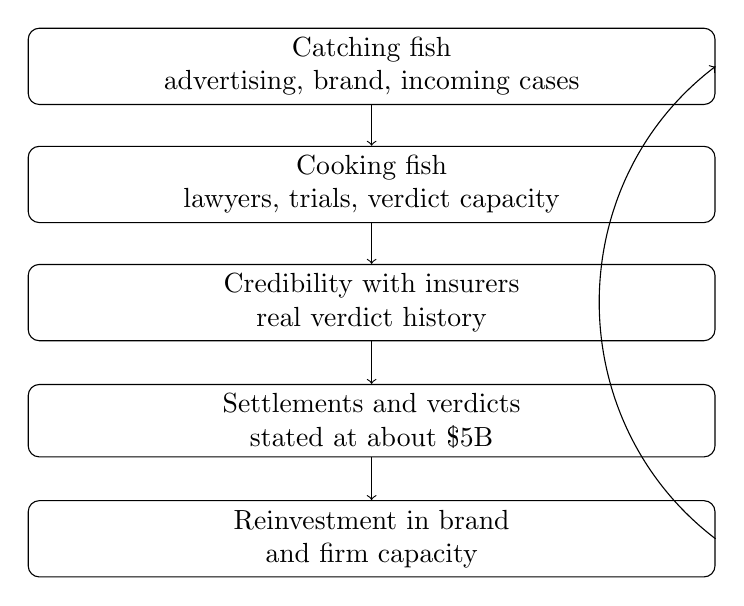
\begin{tikzpicture}[x=1cm,y=1cm]
\node[draw, text width=.70\linewidth, align=center, rounded corners] (ad) at (0,0) {Catching fish\\ advertising, brand, incoming cases};
\node[draw, text width=.70\linewidth, align=center, rounded corners] (law) at (0,-1.5) {Cooking fish\\ lawyers, trials, verdict capacity};
\node[draw, text width=.70\linewidth, align=center, rounded corners] (cred) at (0,-3.0) {Credibility with insurers\\ real verdict history};
\node[draw, text width=.70\linewidth, align=center, rounded corners] (settle) at (0,-4.5) {Settlements and verdicts\\ stated at about \$5B};
\node[draw, text width=.70\linewidth, align=center, rounded corners] (capacity) at (0,-6.0) {Reinvestment in brand\\ and firm capacity};

\draw[->] (ad) -- (law);
\draw[->] (law) -- (cred);
\draw[->] (cred) -- (settle);
\draw[->] (settle) -- (capacity);
\draw[->] (capacity.east) .. controls (2.4,-4.5) and (2.4,-1.5) .. (ad.east);
\end{tikzpicture}
\caption{The operating loop implied by Morgan's catching-fish/cooking-fish metaphor. Marketing without trial capacity is a ``paper tiger''; legal capacity without distribution does not create the same scale.}
\end{figure}

Morgan states that every week the firm has about 200 trial dockets in America:

\begin{equation}
d_{\mathrm{trial\ dockets}} \approx 200\ \mathrm{per\ week}.
\end{equation}

That number matters because it connects advertising to credibility. Marketing creates demand, but trial readiness makes the demand valuable. Without the lawyers, he says, the firm is a paper tiger.

\begin{table}
\centering
\begin{tabular}{|p{.44\linewidth}|p{.44\linewidth}|}
\hline
Transcript-backed quantity & Role in the mechanism\\
\hline
\(\$1.5\mathrm{B}\) Forbes-attributed net worth & Opening status claim\\
\hline
\(\$2\mathrm{B}\) annual fees & Scale of firm economics\\
\hline
\(\$400\mathrm{M}\) advertising & Client acquisition engine\\
\hline
\(\$5\mathrm{B}\) settlements and verdicts & Outcome scale attached to legal execution\\
\hline
\(200\) weekly dockets & Trial readiness and pressure on opponents\\
\hline
\(50\) states, \(24/7\) & Distribution and availability model\\
\hline
\(4\%\) to \(4.5\%\) tax-free bond yield & Wealth-preservation allocation claim\\
\hline
\end{tabular}
\caption{Selected numerical claims from the interview. These are used as source-grounded business arithmetic, not independent verification.}
\end{table}

\section{Keeping Money: Greed, Black Swans, No Debt, and Giving}

Once the interview has established how the firm makes money, it turns to keeping money. Morgan says it is hard to make money and harder to keep it. His stated danger is greed: doing something one knows is wrong because the promise is too attractive. His rule is that if something is too good to be true, it is too good to be true.

The investment sequence is conservative. He mentions \emph{A Random Walk Down Wall Street} and \emph{Black Swan}. He says he uses index funds for equities, tax-free bonds yielding about 4 to 4.5 percent, U.S. Treasuries, and operating assets he understands: attractions, hotels, shopping centers, and apartments. Once money goes into investments, he says, he never touches it.

We can summarize the allocation as a transcript-grounded set:

\begin{equation}
\mathcal{P}
=
\{\mathrm{index\ funds},\ \mathrm{tax\mbox{-}free\ bonds},\ \mathrm{Treasuries},\ \mathrm{owned\ operating\ assets}\}.
\end{equation}

The risk rule from \emph{Black Swan} is even simpler. Morgan's takeaway is not a technical theory of fat-tailed distributions. It is preparedness:

\begin{equation}
\mathrm{Preparedness}
=
\mathrm{savings}
+
\mathrm{no\ debt}
+
\mathrm{readiness\ for\ discontinuity}.
\end{equation}

He is especially forceful about leverage. Debt and leverage, he says, are the death of most business people. He compares leverage to musical chairs: one day the music stops, and the question is whether one has a chair.

The final turn is ethical rather than numerical. For branding, he says one must make the creative creative, build trust for the long haul, and show why hiring the firm makes the client a winner. For a final guiding principle, he gives the golden rule. Then, when asked about advice from his network, he names \emph{Give and Take}: most people are takers, but those who give without expecting anything often end up receiving the most.

So the closing formula is not a financial trick. It is a loop from trust to opportunity:

\begin{equation}
\mathrm{Giving}
\longrightarrow
\mathrm{trust}
\longrightarrow
\mathrm{relationships}
\longrightarrow
\mathrm{opportunity}.
\end{equation}

This completes the lecture's arc. The interview begins with the spectacle of a billionaire lawyer, but the mechanism it leaves us with is more exacting: shared upside, mission, distribution, trial capacity, reputation, no debt, and generosity as long-term infrastructure.

\section{Summary}

The interview gives a practical model of wealth built from a profession. Morgan's path, as presented in the transcript, does not reduce to being a lawyer. It combines a contingency-fee business model, trusted partners, emotionally durable purpose, national distribution, aggressive advertising, real trial capacity, and conservative personal risk management.

The central arithmetic is simple but revealing: \$400 million of advertising is compared with \$5 billion in settlements and verdicts, giving an 8 percent ratio. The central mechanism is more important than the ratio: catching fish requires marketing, cooking fish requires lawyers, and the firm needs both. The final discipline is preservation. Morgan's rules are to avoid greed, avoid what he does not understand, prepare for the Black Swan, carry no debt, keep one's word, and give more than one tries to take.